\documentclass{standalone}
\usepackage{pgfplots}
\usepackage{tikz}%
\pgfplotsset{compat=1.17}

\usetikzlibrary{positioning}%
\begin{document}
	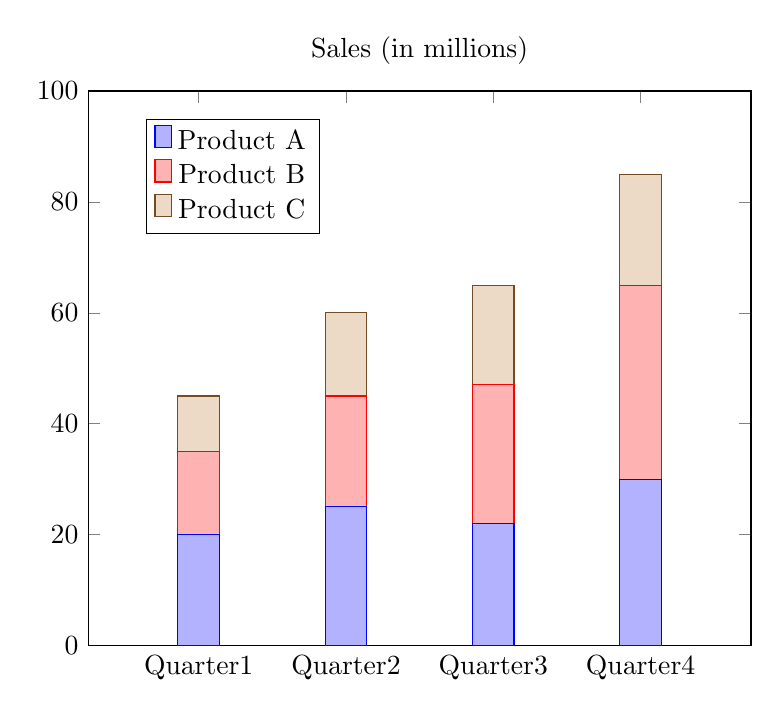
\begin{tikzpicture}
		\begin{axis}[
			ybar stacked,
			name=barchart,
			bar width=15pt,
			enlarge x limits=0.25,
			legend style={
				at={
					(0.35,0.95)
				}
			},
			title={Sales (in millions)},
			symbolic x coords={Quarter1, Quarter2, Quarter3, Quarter4},
			xtick=data,
			ymin=0,
			ymax=100,
			width=10cm
			]
			\addplot + [ybar] plot coordinates {
				(Quarter1,20)
				(Quarter2, 25)
				(Quarter3, 22)
				(Quarter4, 30)
			};
			\addplot + [ybar] plot coordinates {
				(Quarter1, 15)
				(Quarter2, 20)
				(Quarter3, 25)
				(Quarter4, 35)
			};
			\addplot + [ybar] plot coordinates {
				(Quarter1, 10
				)(Quarter2, 15)
				(Quarter3, 18)
				(Quarter4, 20)
			};			
			\legend{Product A,Product B,Product C}
		\end{axis}
	\end{tikzpicture}
\end{document}
